\documentclass[handout]{beamer}
%\documentclass[presentation]{beamer}

\usecolortheme{Waves}
 
\usepackage[utf8]{inputenc}
%\usepackage[UKenglish]{babel}
\usepackage{booktabs}
\usepackage{caption}
\usepackage{subcaption}
\usepackage{array,ragged2e}
\usepackage{graphicx}
\usepackage{amsmath}
\usepackage{amsfonts}
\usepackage{amssymb}
\usepackage{epstopdf}
\usepackage{xmpmulti}
\usepackage{beamerbasethemes}
\usepackage{calc}
\usepackage{ifthen}
\usepackage{graphics}
\usepackage{nicefrac}
\usepackage{xcolor}
\usepackage{calc}
\usepackage{tikz}


\newenvironment{colortheme}[1]{
\def\ProvidesPackageRCS $##1${\relax}
\renewcommand{\DeclareOption[2]}{\relax}
\renewcommand{\ProcessOptions}{\relax}
\makeatletter
\input beamercolorthemeWavesDark.sty
\makeatother
}{}

\setbeamertemplate{footline}[text line]{%
  \parbox{\linewidth}{\vspace*{-8pt}Incoherent Mapping of the GWB\hfill\insertshortauthor\hfill\hfill\insertpagenumber}}
\setbeamertemplate{navigation symbols}{}

%\setbeamertemplate{footline}[frame number]

\usepackage[font={scriptsize},labelfont=bf]{caption}

\usepackage{tikz}
\usetikzlibrary{mindmap,trees}
\pgfdeclarelayer{background}
\pgfdeclarelayer{foreground}
\pgfsetlayers{background,main,foreground}

\usepackage[english]{babel}
\usepackage{amsmath,bm,dsfont,amssymb}
\usepackage{csquotes}
%\usepackage[square,sort,comma,numbers]{natbib}
\usepackage{float,placeins}
\usepackage{wasysym}	
\usepackage{xcolor,transparent}
\usepackage[toc,page]{appendix}

\usepackage{enumerate}
\usepackage{import}
\usepackage{bbold}
%\graphicspath{{graphics/}}
\newcount\colveccount
\newcommand*\colvec[1]{
        \global\colveccount#1
        \begin{pmatrix}
        \colvecnext
}
\def\colvecnext#1{
        #1
        \global\advance\colveccount-1
        \ifnum\colveccount>0
                \\
                \expandafter\colvecnext
        \else
                \end{pmatrix}
        \fi
}
\newcommand{\ra}{\rightarrow	}
\newcommand{\vt}{\vartheta	}
\newcommand{\bs}{\boldsymbol}
\newcommand{\vp}{\varphi}
\newcommand{\de}{\partial}
\newcommand{\Tr}{\mathrm{Tr}}
\newcommand{\csec}{\mathrm{csec}}
\newcommand{\ctan}{\mathrm{ctan}}
\newcommand{\G}{\mathsf{G}}
\newcommand{\F}{\mathsf{F}}
\newcommand{\atan}{\mathrm{atan}}

\newcommand\Wider[2][3em]{%
\makebox[\linewidth][c]{%
  \begin{minipage}{\dimexpr\textwidth+#1\relax}
  \raggedright#2
  \end{minipage}%
  }%
}

\usepackage{hyperref}
\usepackage{url}
\usepackage{animate}

% complying UK date format, i.e. 1 January 2001
\usepackage{datetime}
\let\dateUKenglish\relax
\newdateformat{dateUKenglish}{\THEDAY~\monthname[\THEMONTH] \THEYEAR}

% Imperial College Logo, not to be changed!
\institute{
\includegraphics[height=0.7cm]{LOGO.pdf}}

% -----------------------------------------------------------------------------
%\setbeamertemplate{title page}[default]
\setbeamercolor{title}{bg=}
\setbeamercolor{subtitle}{bg=}
%\setbeamertemplate{blocks}[default]
\setbeamercolor{date}{bg=}
%\setbeamertemplate{blocks}[default]
\setbeamercolor{block title}{bg=}
\setbeamercolor{block body}{bg=black}
 \definecolor{textcol}{HTML}{83DFD3} 

 \definecolor{namecol}{HTML}{A6F6EC}
 \definecolor{textcol2}{HTML}{E1D5AF}
  \definecolor{textcol1}{HTML}{FF7604}
\usebackgroundtemplate%
{%
    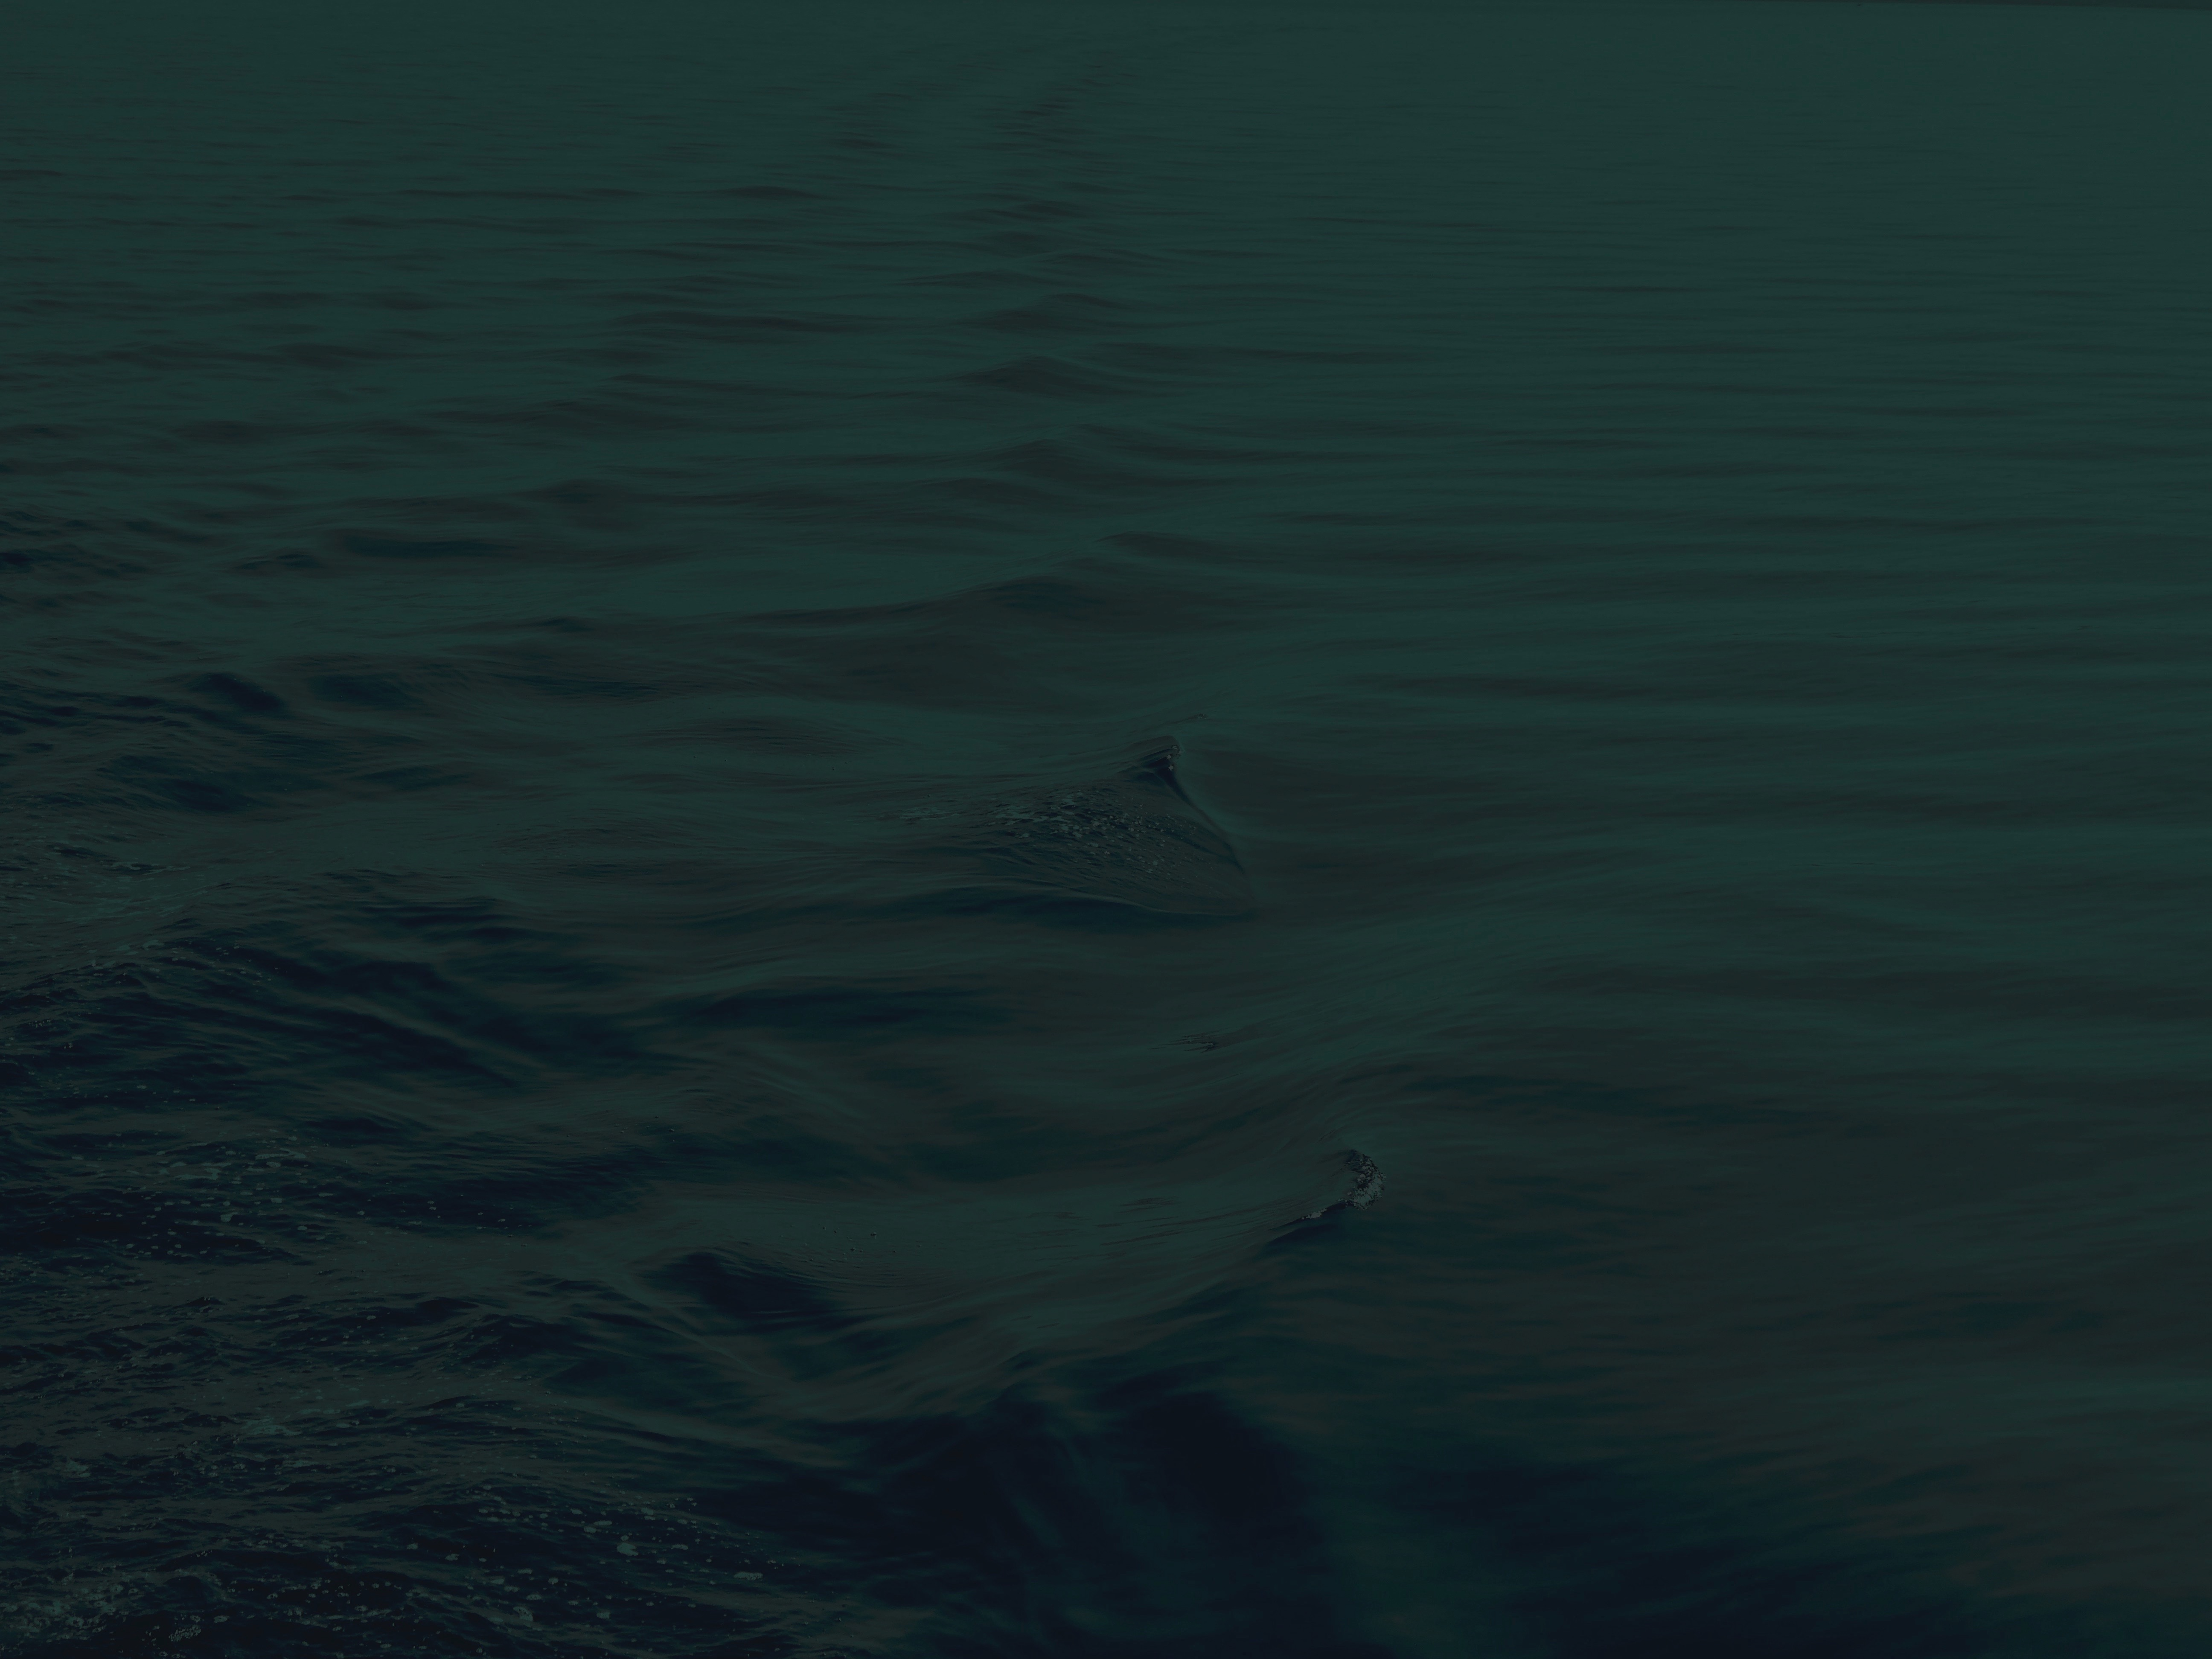
\includegraphics[width=\paperwidth,height=\paperheight]{bkd.jpg}%
}



%Information to be included in the title page:
\title{\textcolor{white}{\bf Mapping the Incoherent Gravitational Wave Background}}

\subtitle{\textcolor{white}{Using multiple ground-based interferometers}}

\author[Arianna I. Renzini]{\textcolor{namecol}{\textbf{Arianna I. Renzini}, Carlo R. Contaldi\\
arXiv:1806.11360}}
\date{\textcolor{textcol}{\today}}



\setbeamertemplate{blocks}[rounded][shadow=false]
\addtobeamertemplate{block begin}{\pgfsetfillopacity{0.5}}{\pgfsetfillopacity{1}}

\begin{document}

\frame{\titlepage}

\begin{frame}
	%\frametitle{Introduction: what is the GWB?}
    
			\centering
			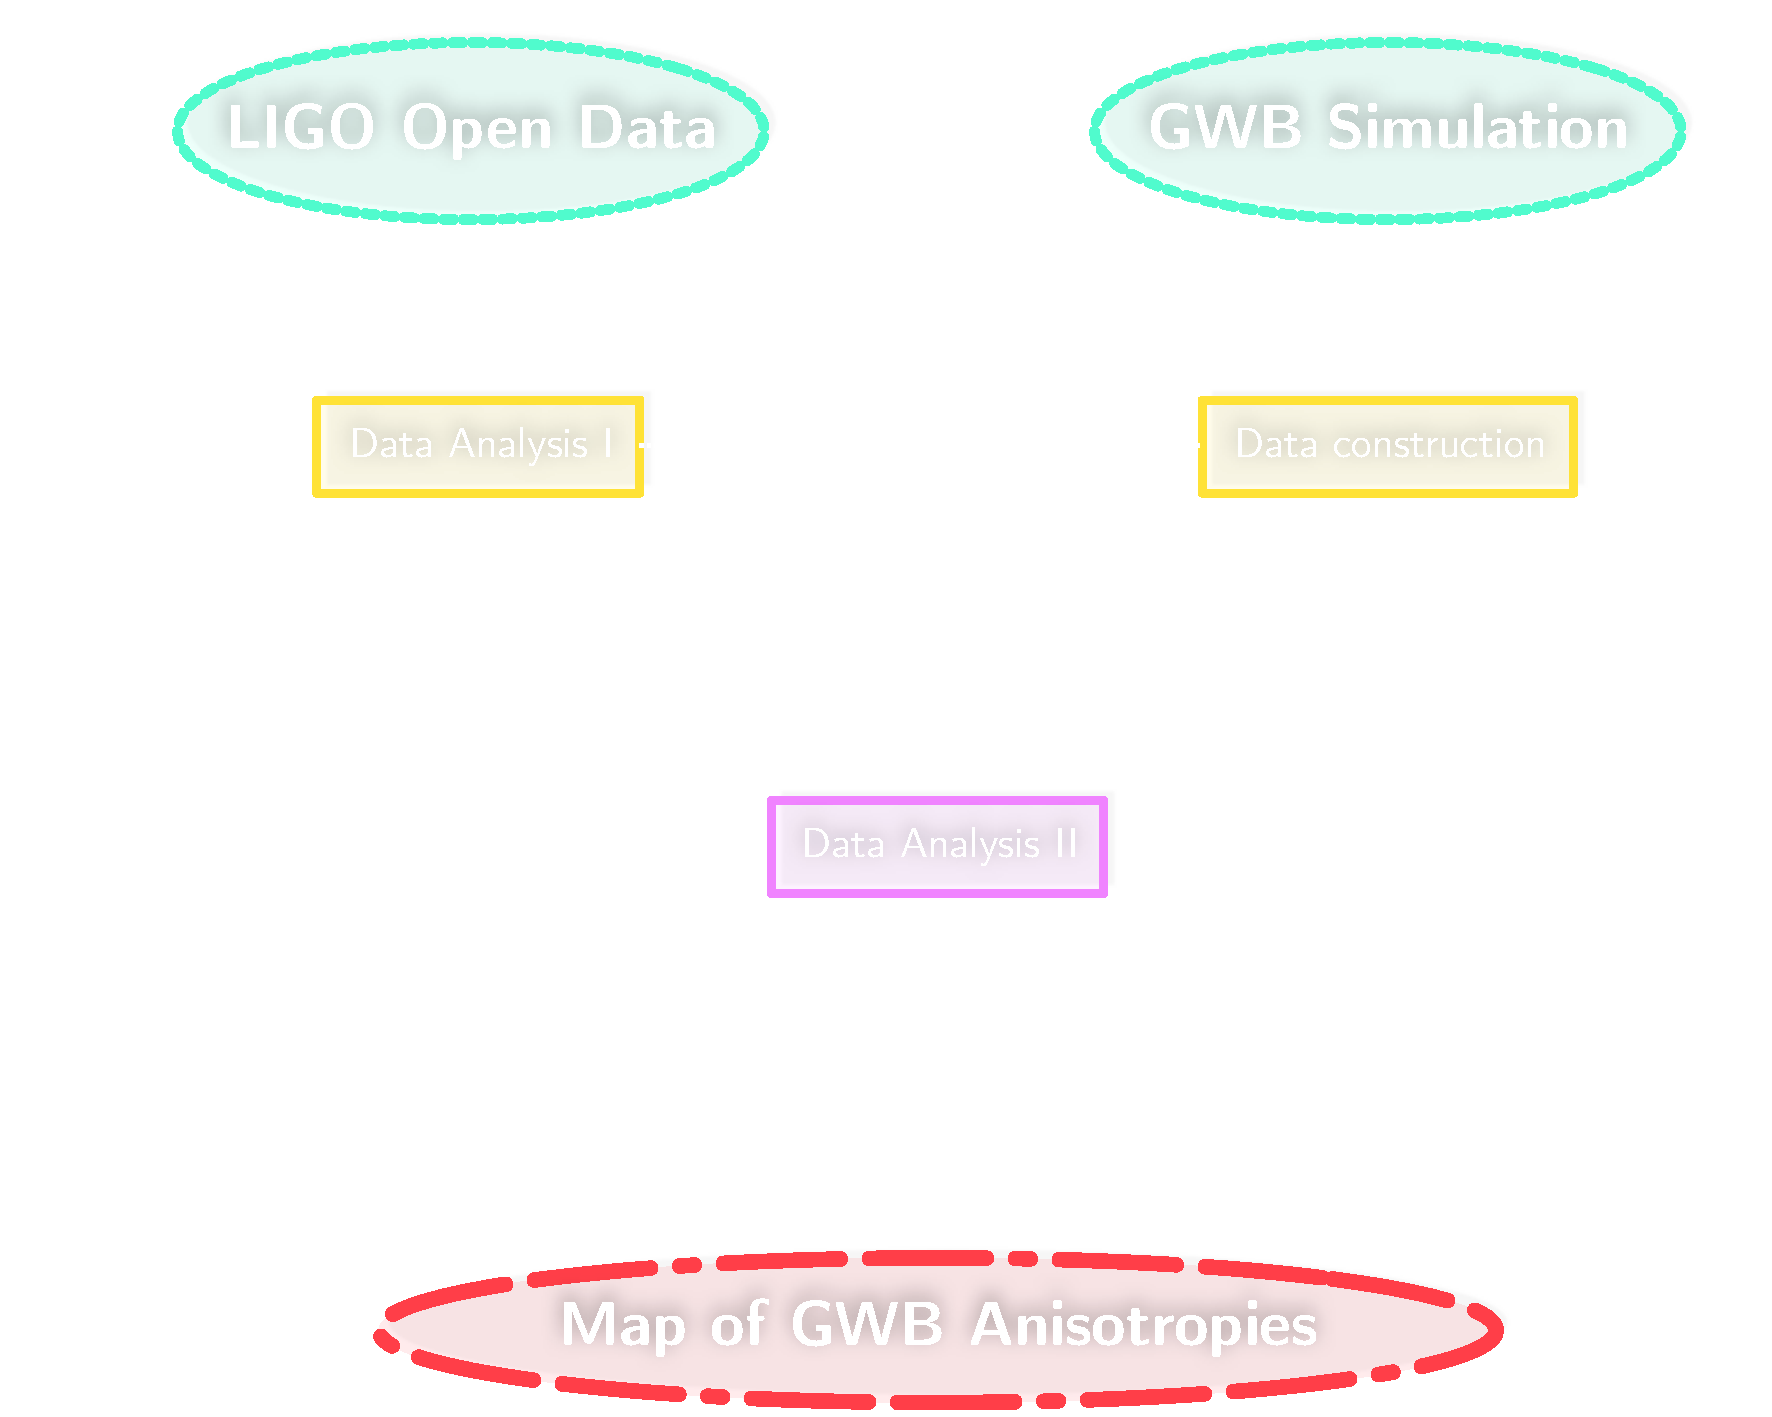
\includegraphics[width=0.95\textwidth]{flow.pdf}




\end{frame}


\begin{frame}
	\frametitle{Introduction: what is the GWB?}
	     	\smallskip
   {\bf Unresolved} signals of \textcolor{textcol}{\bf Astrophysical} or \textcolor{textcol}{\bf Cosmological} nature:\\
   \medskip
    %	\begin{figure}[h]
			\centering
			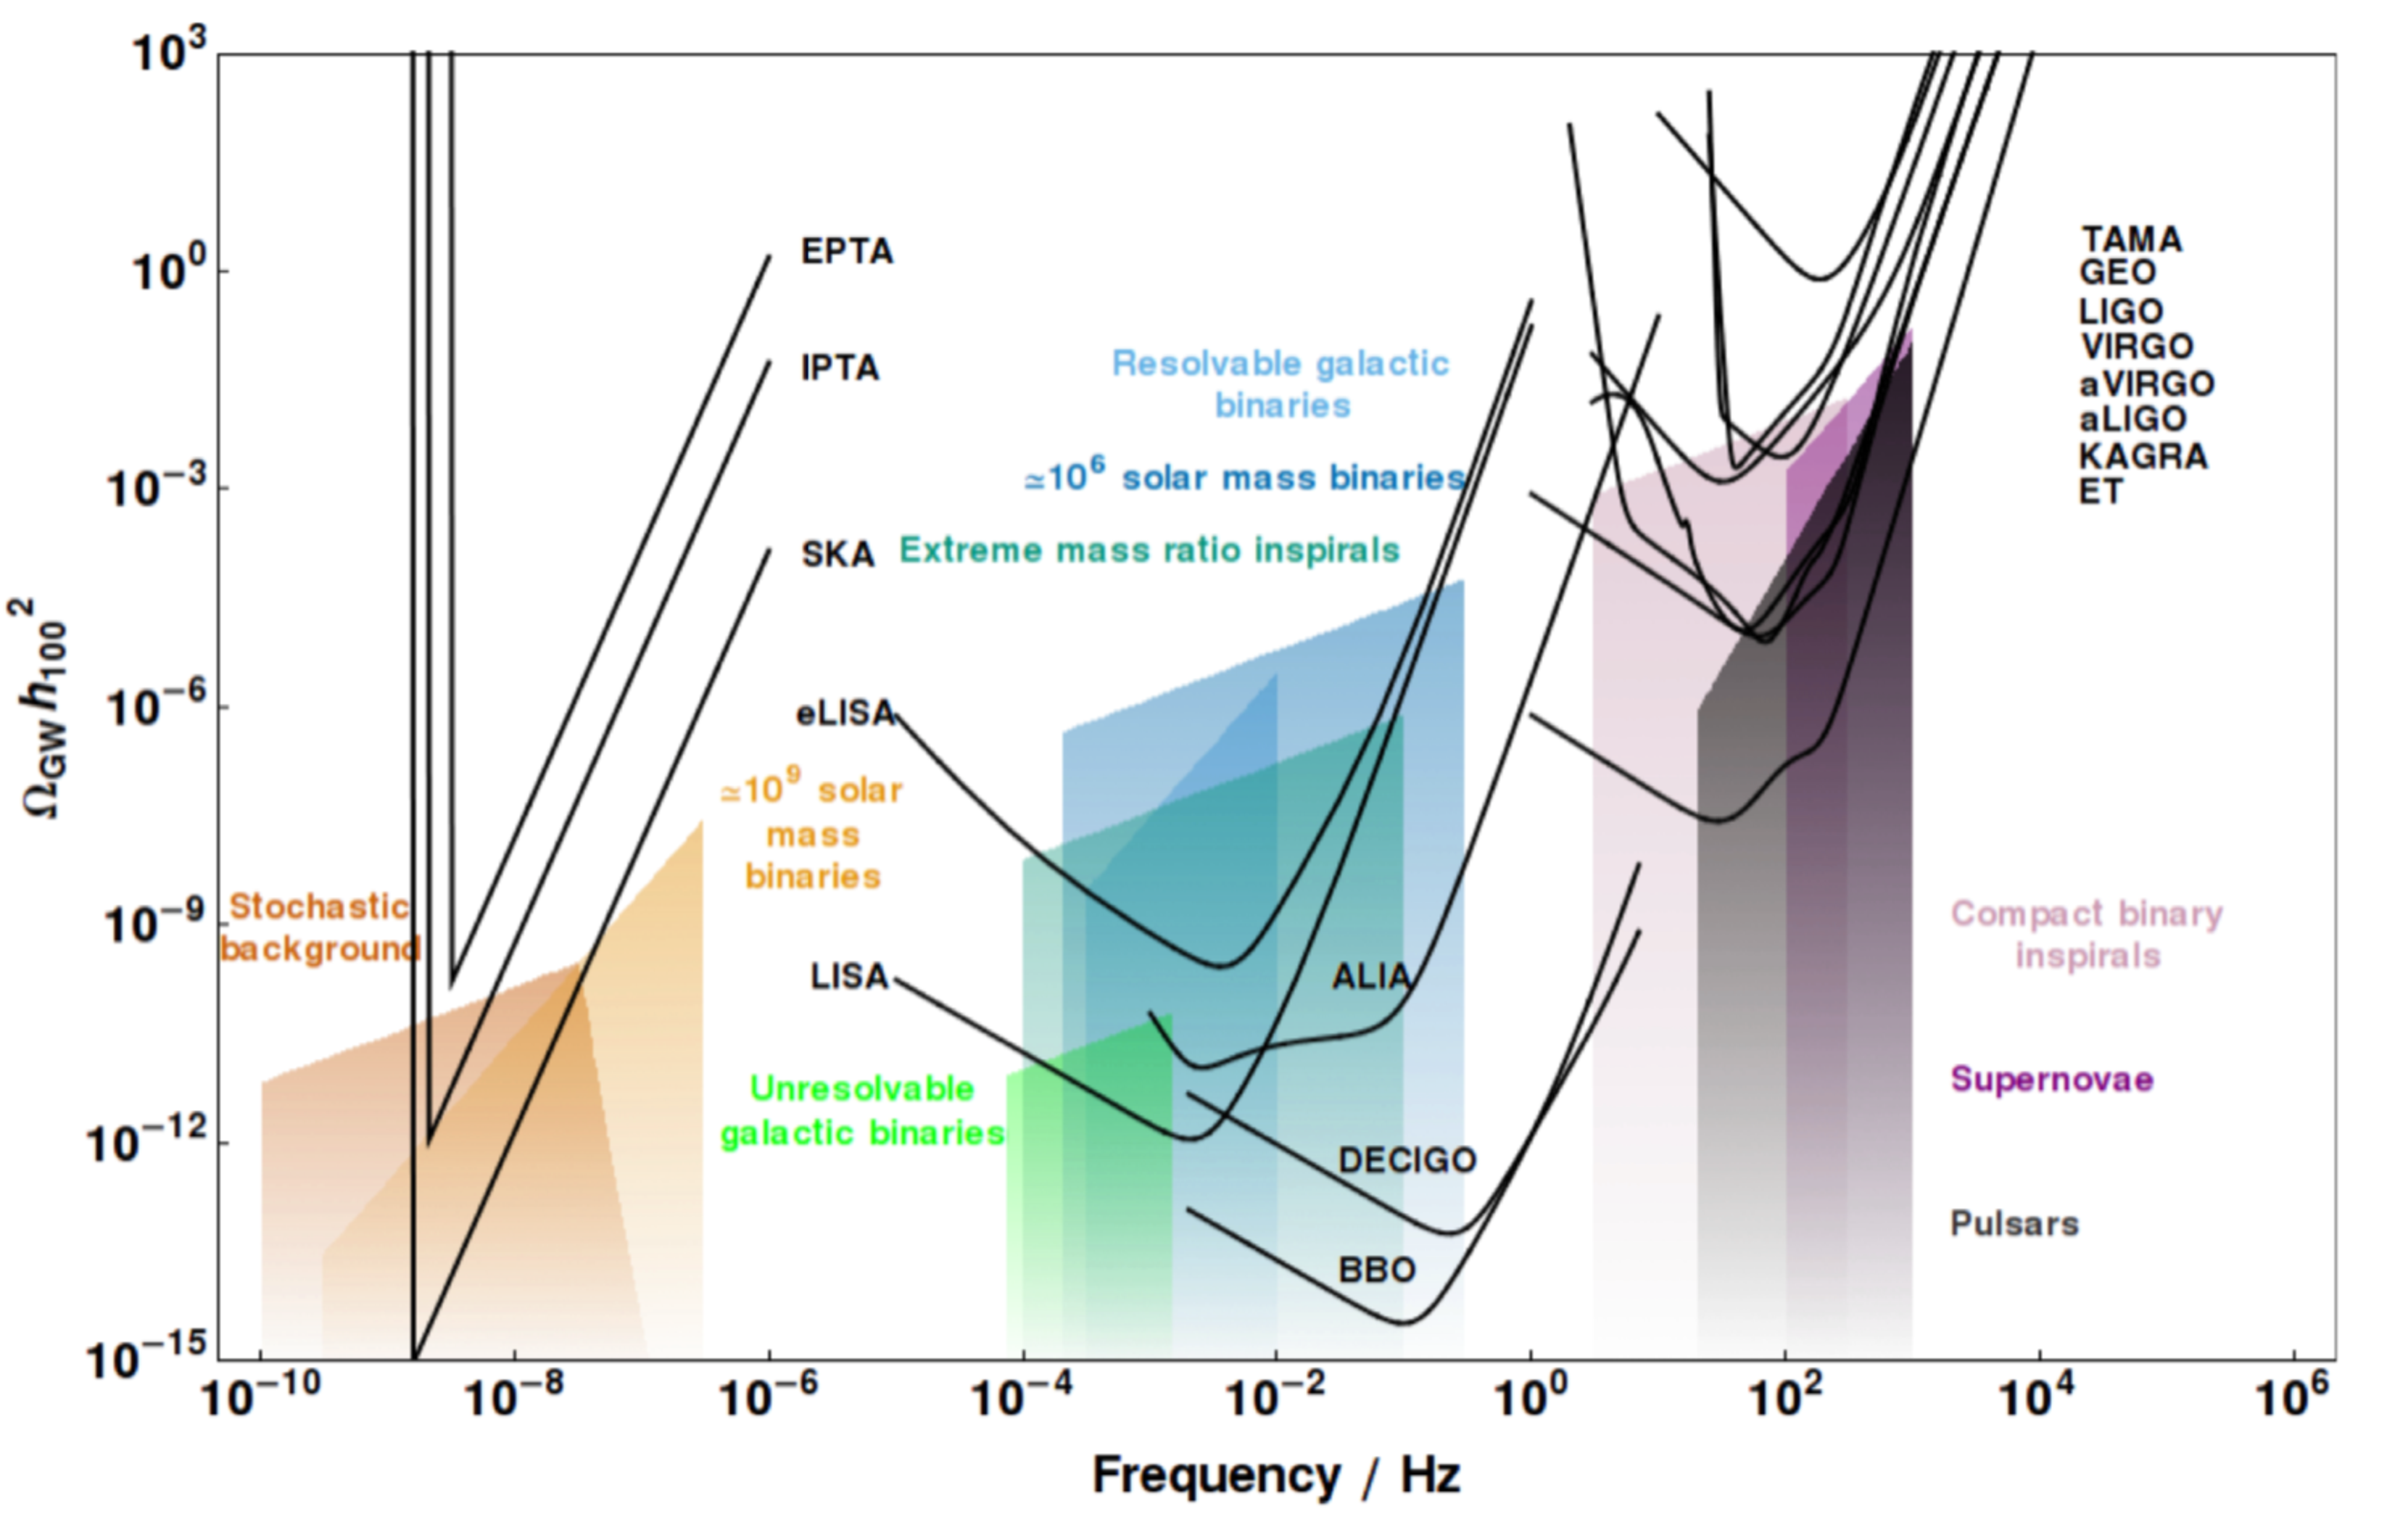
\includegraphics[width=0.67\textwidth]{GWBplots.pdf}\\
			%\scriptsize
			%\caption{Current constraints on the GWB and models, from [Moore et al., 2014].}
			%\label{output}
		%\end{figure}
\smallskip
     	Energy spectrum [Allen and Romano, 1999]:\\
     	\smallskip
$
			\Omega_{GW}(f) = \frac{1}{\rho_c} \frac{d\rho_{GW}}{d\ln f}=  \frac{16\pi^3}{3 H_0^2}f^3\, I(f)
$
\tiny
\flushright  [Image Credit: Moore et al., 2014]

%DETECTING THESE WILL HAVE BIG PHYSICAL IMPLICATIONS

\end{frame}


\begin{frame}
	\frametitle{Objectives and motivation}
    	
        The goal is to {\bf map gravitational wave anisotropies on the sky}, using {\bf all available data} from online detectors and future ones.\\
        \medskip
        \begin{description}
\item[\textcolor{textcol}{Astro-GWB}] Investigate large scale structure, polarisation  \textcolor{textcol1}{\bf guaranteed detection $^\star$}
\item[\textcolor{textcol}{Cosmo-GWB}]  Constrain cosmological models - not in band...

\end{description}
        

%    \begin{center}
%    Limit for inspiral-dominated GWB [Abbott et al., 2017]: $$\Omega_{2/3}(\bm{n}) < 2 - 6 \times 10^{-8} \,\text{sr}^{-1} $$
%     \end{center}
    % obtained in a specific, 2-detector frame. The multiple baseline search needs a more general frame and will be more constraining.
\small
\medskip
Current limits on $\Omega_{GW}$ [Abbott et al., `17 \& Arzoumanian et al., `18]:\\
\medskip
\centering
\begin{tabular}{l | c | c  }
GWB type & PTAs \quad ($f\sim nHz$)& LIGO  \quad ($f\sim 10 \,Hz$) \\
\hline \hline
astro& -& $ 1.7 \times 10^{-8}$\\
inspiral& $3.58\times 10^{-9}$& $1.3 \times 10^{-7}$\\
cosmo& $7.6 \times 10^{-10}$ &  $1.7 \times 10^{-7}$\\
\end{tabular}
\flushleft
95\% upper limits.\\
\smallskip
\scriptsize
\textcolor{textcol1}{$^\star$} given detection results and integration times
\end{frame}

\begin{frame}[plain]
\textcolor{white}{Many GWB mappers have used simplyfying constraints:}\\
\centering
\medskip
\textcolor{textcol2}{sidereal folding       -       coherent approaches       -        radiometer maps}
\flushleft
\medskip
\textcolor{white}{Our approach is similar to \textcolor{textcol2}{spherical harmonic decompositon} + \textcolor{textcol2}{CMB tools}; keywords:}
\medskip

\begin{minipage}{0.3\textwidth}
\hfill
\vskip 1.5cm 
\end{minipage}
\begin{minipage}{0.35\textwidth}
\centering
\textcolor{white}{
\textbf{pixel space} \\
 \textbf{sky coordinates}\\
  \textbf{$\sim$ any signal}\\
  \textbf{long integration time}
  }
  \end{minipage}
\begin{minipage}{0.3\textwidth}
\flushleft
\footnotesize
\textcolor{textcol}{ \bf \bf{\Big\}}generalised pointing}\\
\normalsize
\vskip 0.65 cm
\textcolor{blue!50!black}{\\.}
\end{minipage}
\flushleft
% but we work in \textbf{pixel space} and \textbf{sky coordinates}. Assume $\sim$nothing about the signal - based on  the \textbf{long integration times} available.}\\
%but how is it different, substantially, from the Ylm decomp approach?
\medskip
\textcolor{white}{Here we concentrate on LIGO/Virgo detectors, building a pipeline based on real data to reconstruct a GWB  map.}\\
\bigskip
\textcolor{white}{The approach is general and may be extended to other detectors.}\\
\smallskip
%\textcolor{textcol}{\textbf{especially useful for LISA:} basis for an iterative map-maker - needed as signal will bias noise }
%We will now extend the algorithm to other detectors (LISA, PTAs).\\

\end{frame}


\begin{frame}
	\frametitle{DATA ANALYSIS I}
	\bigskip
    \begin{minipage}{0.45\textwidth}
			\centering

				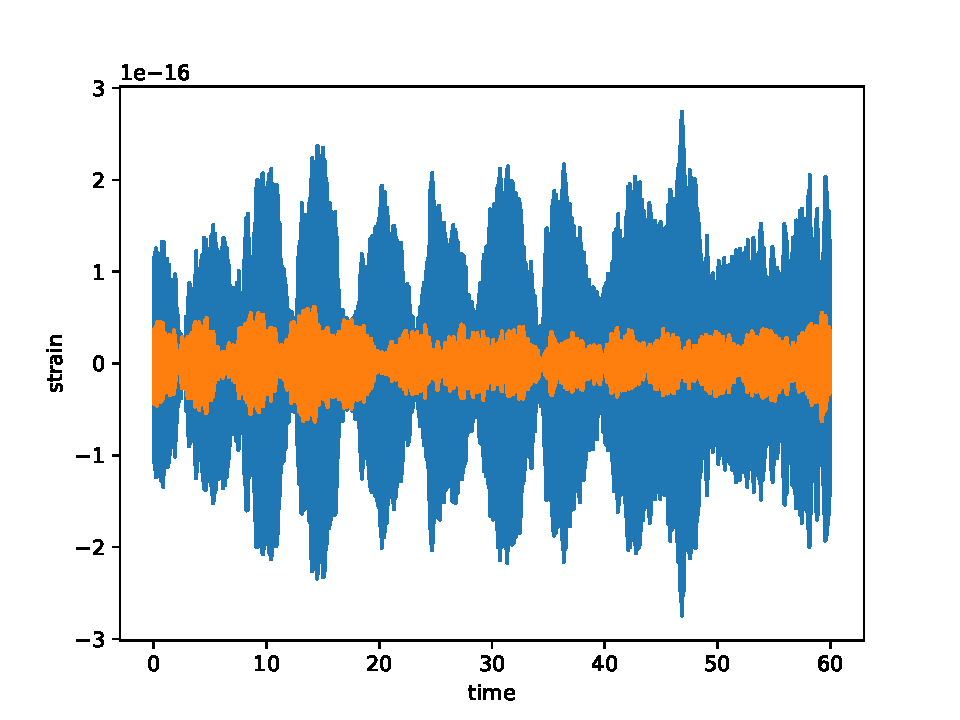
\includegraphics[width=0.95\textwidth]{h1} \
\scriptsize
				Signal in time
\end{minipage}
\hfill
\begin{minipage}{0.45\textwidth}
			\centering
				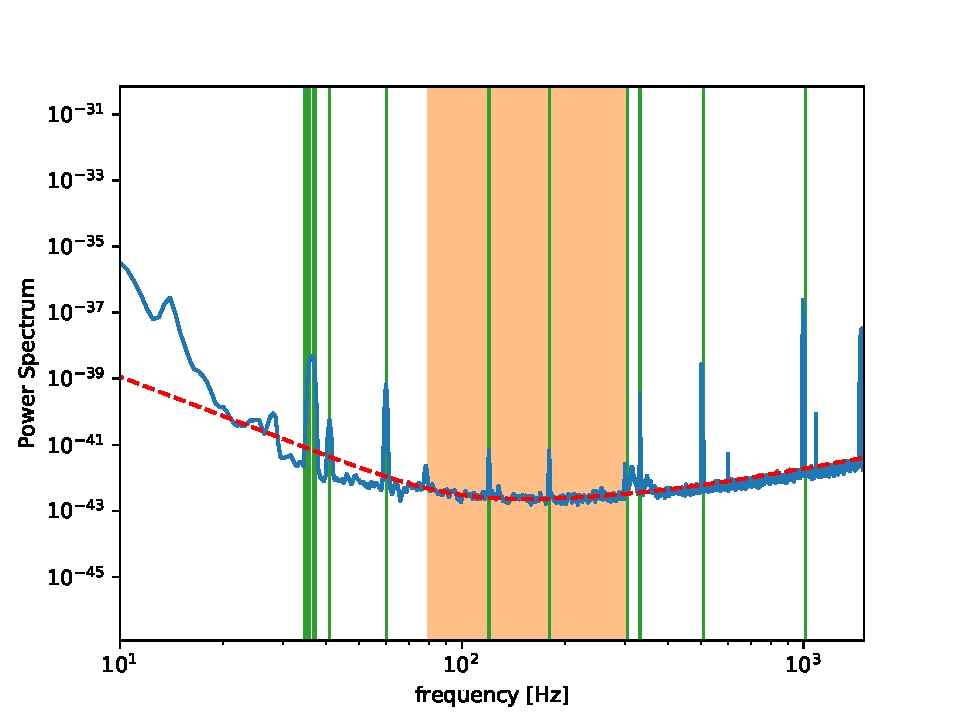
\includegraphics[width=0.95\textwidth]{psd} \
\scriptsize
				Power Spectrum Density
	\end{minipage}\\
	\smallskip
    \centering

\begin{itemize}
\small
    \item[$\bigstar$] flag coincident data chunks and divide into 60 s segments
    \item[$\bigstar$] clean the data: notching $+$ windowing
    \item[$\bigstar$] FFT segments, apply high $+$ low pass filters: [80:300] Hz
    \item[$\bigstar$] fit PSD and discard segments based on parameter estimation
    \begin{block}{}
\centering
\normalsize
\textcolor{textcol}{\bf Result: segments of coincident data in frequency space $s_i(f)$\\
take the cross-correlation $d_{H-L} = s_{LH}^{}\,s_{LL}^\star$.}
\end{block}
\end{itemize}

\end{frame}

\begin{frame}
	\frametitle{DATA CONSTRUCTION}
 The strain measured by detector $i$ may be theoretically written as
  \begin{equation}
s_{i}(f)=\int_S\, d\bm{\hat n}\,\sum_{A=+,\,\times}\,h^{}_A\,(f,\,\bm{\hat n})\,F_i^A\,(f,\,\bm{\hat n})\,e^{i2\pi f\,\bm{n\cdot x}_i}\,
\label{dectresp}
\end{equation}
 \flushleft
$F_+$ and $F_\times$ are the \textbf{polarisation response functions} of the detector.\\
\smallskip
\normalsize 
The cross-correlation of signals from two detectors will be
\begin{equation}
S_{\bm b}(f) = s_i\,s_j^{\star} = \int_{S^2} d\bm{m}\, \gamma_{I,\,\bm{b}}(\bm{m})\,I(f,\,\bm{m})\,e^{2\pi i f \bm{m}\cdot\bm{b}}
\end{equation}
$\gamma_{I, \bm{b}}$ is the \textbf{overlap function} of the \textbf{baseline} $\bm{b}$. \\
\begin{block}{}
\centering
\textcolor{textcol}{\bf We generate $I(f,\bm{m})$ for a GWB and input in (2) to obtain correlated data in frequency space.}
\end{block}
\end{frame}

\begin{frame}
	\frametitle{DATA CONSTRUCTION}
	Real data contains both signal and noise,
     \begin{equation}
	d_{\bm{b}}(f) = S_{\bm{b}}(f)+N_{\bm{b}}(f)
	\end{equation}
    we generate $N_\bm{b}(f)$ as random Gaussian noise with different amplitudes to mimic \textbf{High/Low SNR}. \\
    \smallskip
     $d_{\bm{b}}(f)$ may be generated for any number of baselines $\bm b_i$, building a network of interferometers. \\
    \medskip
    NOTE: in our frame $\bm b$ is time-dependent  $\bm b \equiv \bm b (t)$ $\Rightarrow$
    \begin{block}{}
\centering
\textcolor{textcol}{\bf $d_{\bm{b}}(f)$ is generated for 60 s segments where $\bm b$ is constant. }
\end{block}
\medskip 
The overlap function $\gamma_{I, \bm{b}}$ is rotated minute by minute into sky coordinates:
\end{frame}

{\usebackgroundtemplate%
{%
    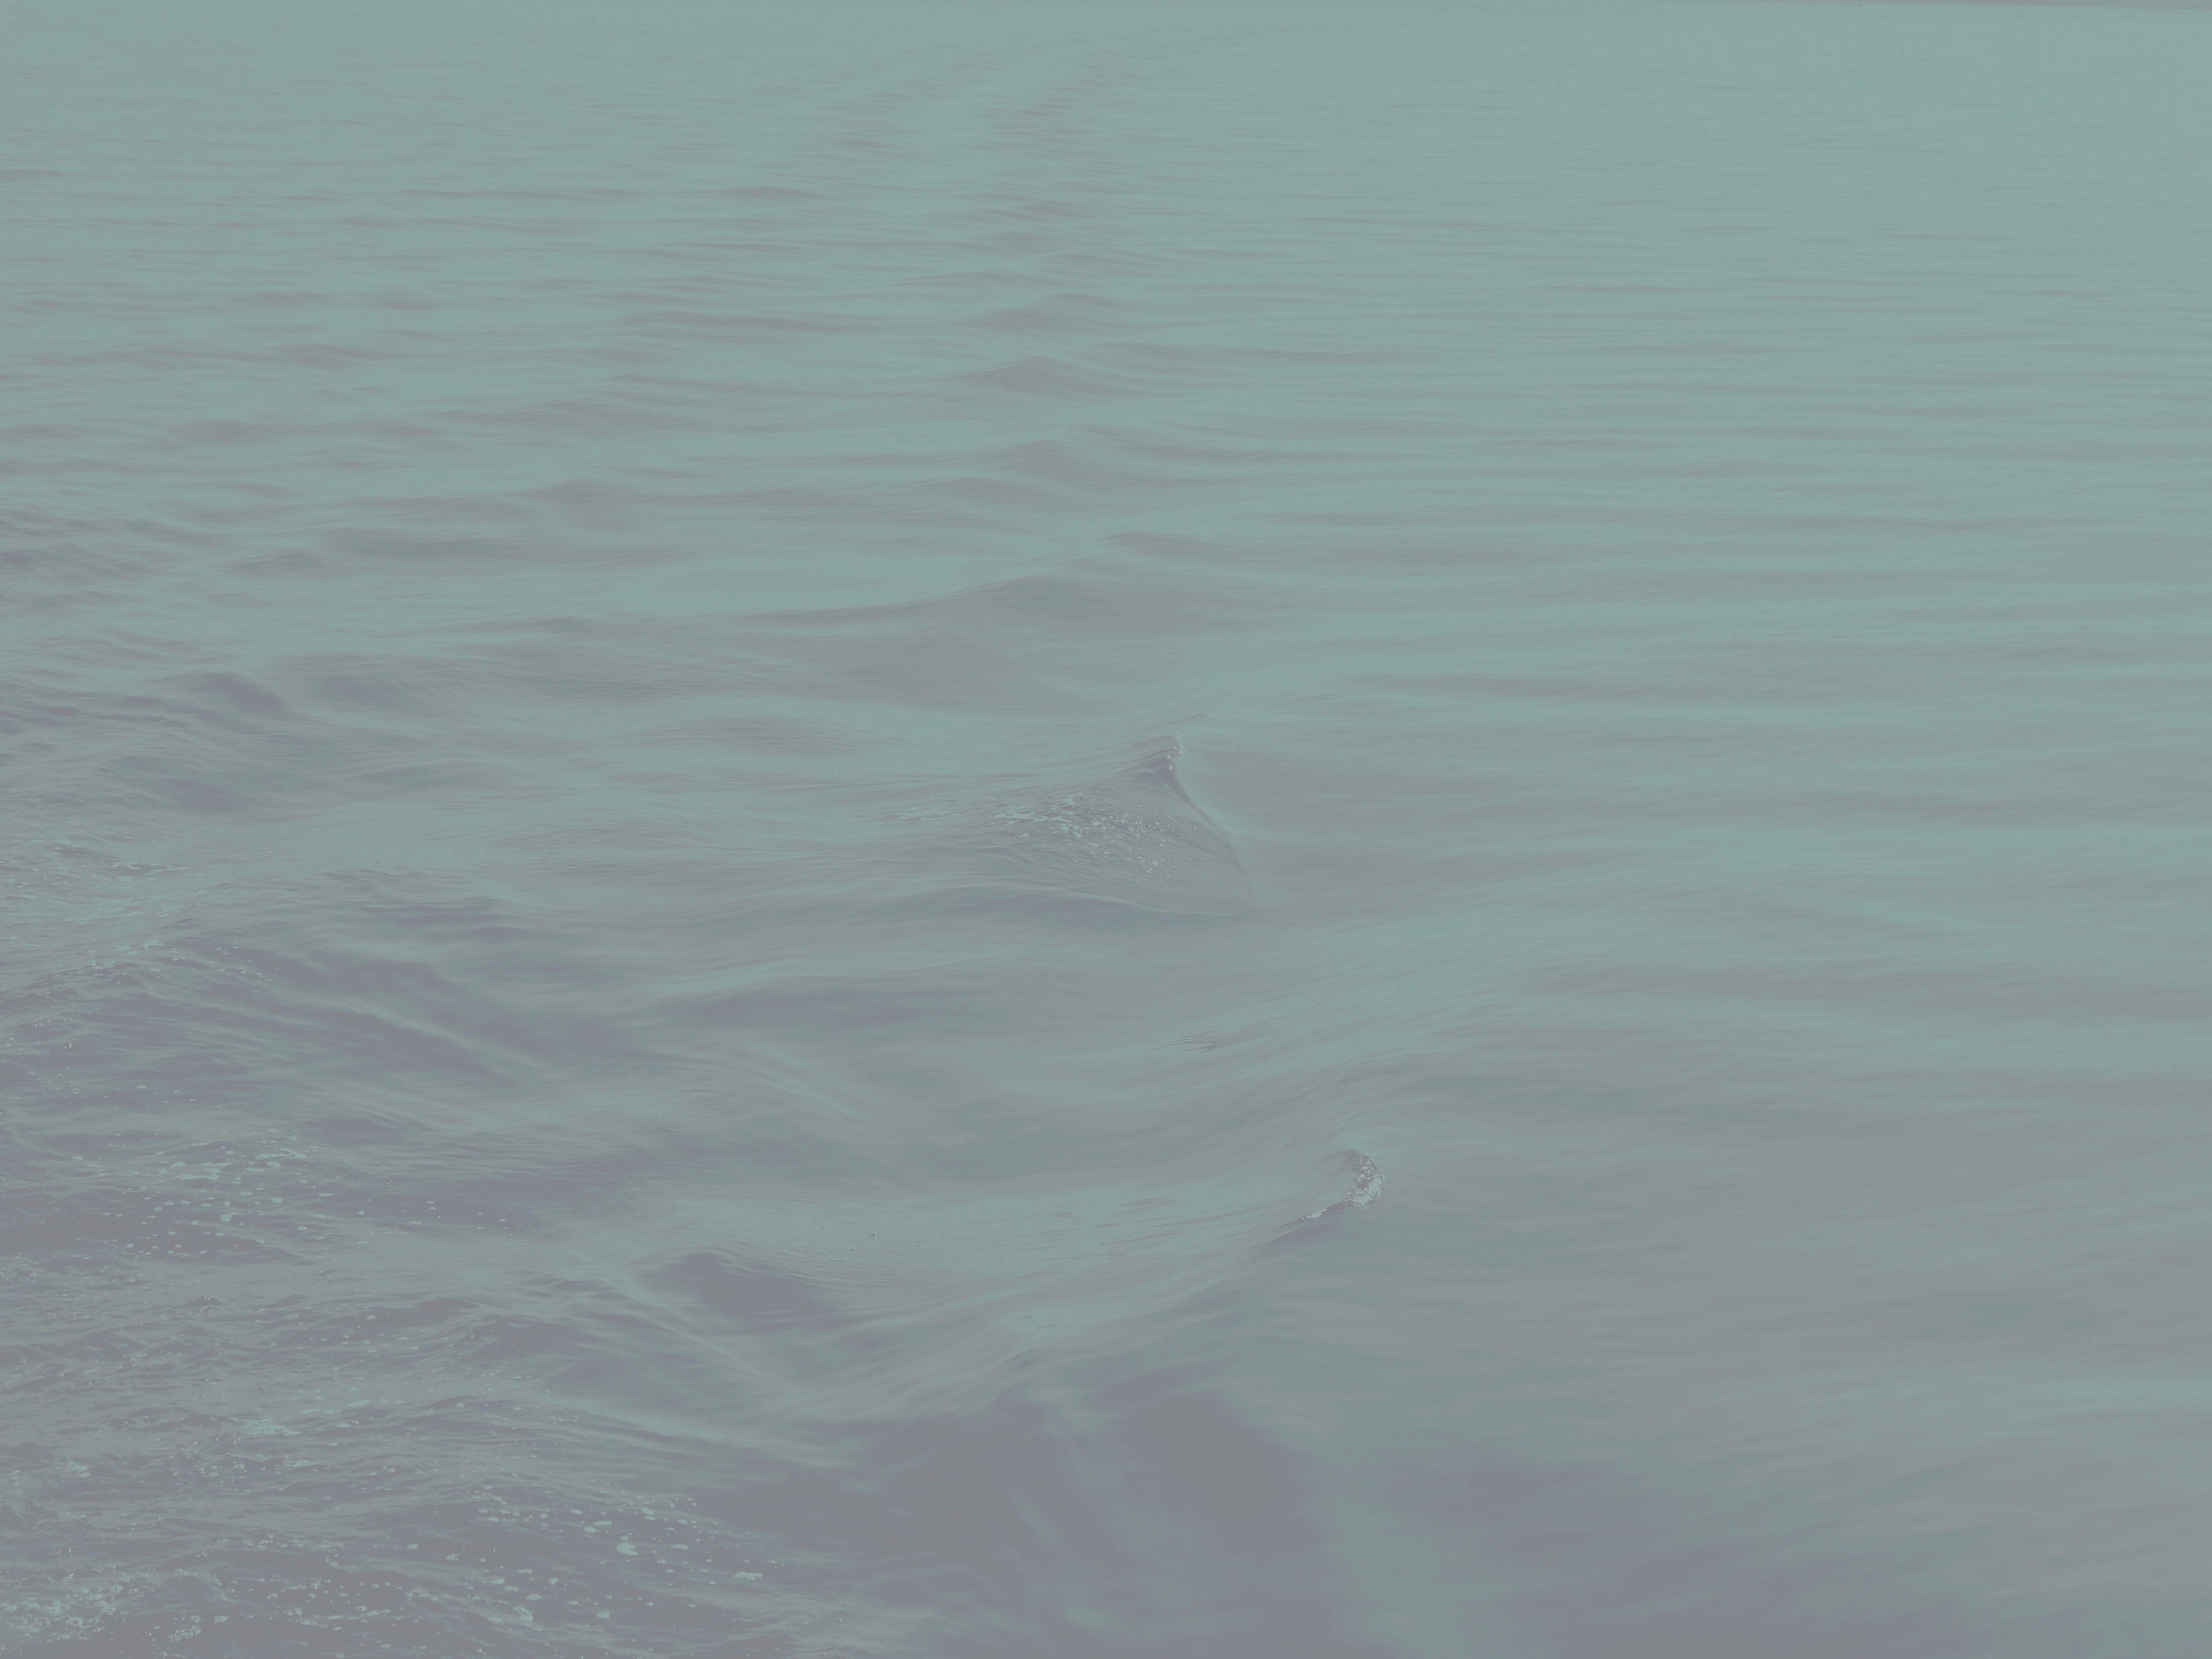
\includegraphics[width=\paperwidth,height=\paperheight]{bklight.jpg}%
}
\begin{frame}[plain]

	\frametitle{\textcolor{black}{$\gamma_I$}}
    
	\begin{figure}
	  \animategraphics[loop,controls,width=0.8\linewidth]{8}{gammaI/gamma_rot}{0}{26} %26
		% remove the 'draft' keyword, when replacing with final figure!
	\caption*{\centering \small \textcolor{black}{The overlap function $\gamma_I$ on the sky for the LIGO detector pair. The scale of the beam sets the reconstruction resolution. Note: peaked $\Rightarrow$ aliasing on large scales.}}
	\end{figure}
    \smallskip

\end{frame}
}
\begin{frame}
	\frametitle{DATA ANALYSIS II}
    We now have segments of correlated data in frequency space, either from the LIGO baseline or generated for $N$ baselines.\\
    
    \begin{block}{}
    \centering
    \textcolor{textcol}{ \bf We extract the \textbf{optimal map} $I(\bm m)$ given the data with a \textbf{maximum likelihood method}: }
    \end{block}
    Minimise the $\chi^2$ of the map given the data [Thrane et al, 2009]
            \begin{equation}
		\chi^2(I_{m}) = -\frac{1}{2} \sum_{t,\,f}\frac{(d_{\bm b}-\langle d_{\bm b}\rangle)(d_{\bm b}-			\langle d_{\bm b}\rangle)^\star}{N(f)}
		\label{chisqu}
		\end{equation}

$$ \langle d_{\bm b}(f)\rangle\equiv S_{\bm b} (f) \qquad N(f) = P_A(f)\,P_B(f)$$

Where $A$, $B$ label the detectors in the baseline $\bm b$. This works as the PSD of the noise is just the PSD of the data $P(f)$.

\end{frame}

\begin{frame}
	\frametitle{DATA ANALYSIS II}
		Defining the \textbf{dirty map} $z_{m}$:
        \begin{equation}
			z_{m} : =\textcolor{textcol}{\sum_{b\,\in \,\text{base}}} \sum_{T\, \in\, \text{block}} \sum_{f}\frac{M_{m}^{I\star}(\hat{b})}{N(f)} d^T(f, \hat{b})\,
			\label{dirtym}
		\end{equation}
		and the \textbf{beam-pattern matrix}:
		\begin{equation}
		A_{mn} :=  \textcolor{textcol}{\sum_{b\,\in \,\text{base}}}\sum_{T\, \in \, \text{block}} \sum_{f}				\frac{M_{n}^I(\hat{b})M_{n}^{I^\star}(\hat{b}) }{N(f)}\,\,\,
		\end{equation}
the \textbf{clean map} solution which maximizes likelihood is 
\begin{block}{}
\textcolor{textcol}{
\begin{equation}
\bm{ I_{n} = \sum_{m}  \left(A_{mn}\right)^{-1} z_{m} }
\end{equation}
}
\end{block}
\end{frame}

\begin{frame}{}
    \textcolor{white}{The beam-pattern matrix for 1 baseline isn't easily invertible; the more baselines the better the conditioning of the matrix is.}\\
\bigskip
\textcolor{white}{Naturally, the conditioning gets better over integration time.}\\
\bigskip
The code is set up to\\
\smallskip
\textcolor{textcol}{\bf A. Create input from multiple detectors on earth } \\
\textcolor{textcol}{\bf B. Integrate over long periods of time }\\
        \medskip
        \centering
        hence\\
        \smallskip
\flushleft
		    \textcolor{textcol1}{{\bf TEST A.} Simulate correlated data for different baselines: }\\
		    			\medskip
			\centering
			\textcolor{textcol1}{\bf LIGO L \quad$-$\quad LIGO H  \quad$-$\quad Virgo}\\
			\medskip

			\textcolor{textcol1}{{\bf TEST B.} Analyse the whole LIGO O1 open data}\\


\end{frame}

{\usebackgroundtemplate%
{%
    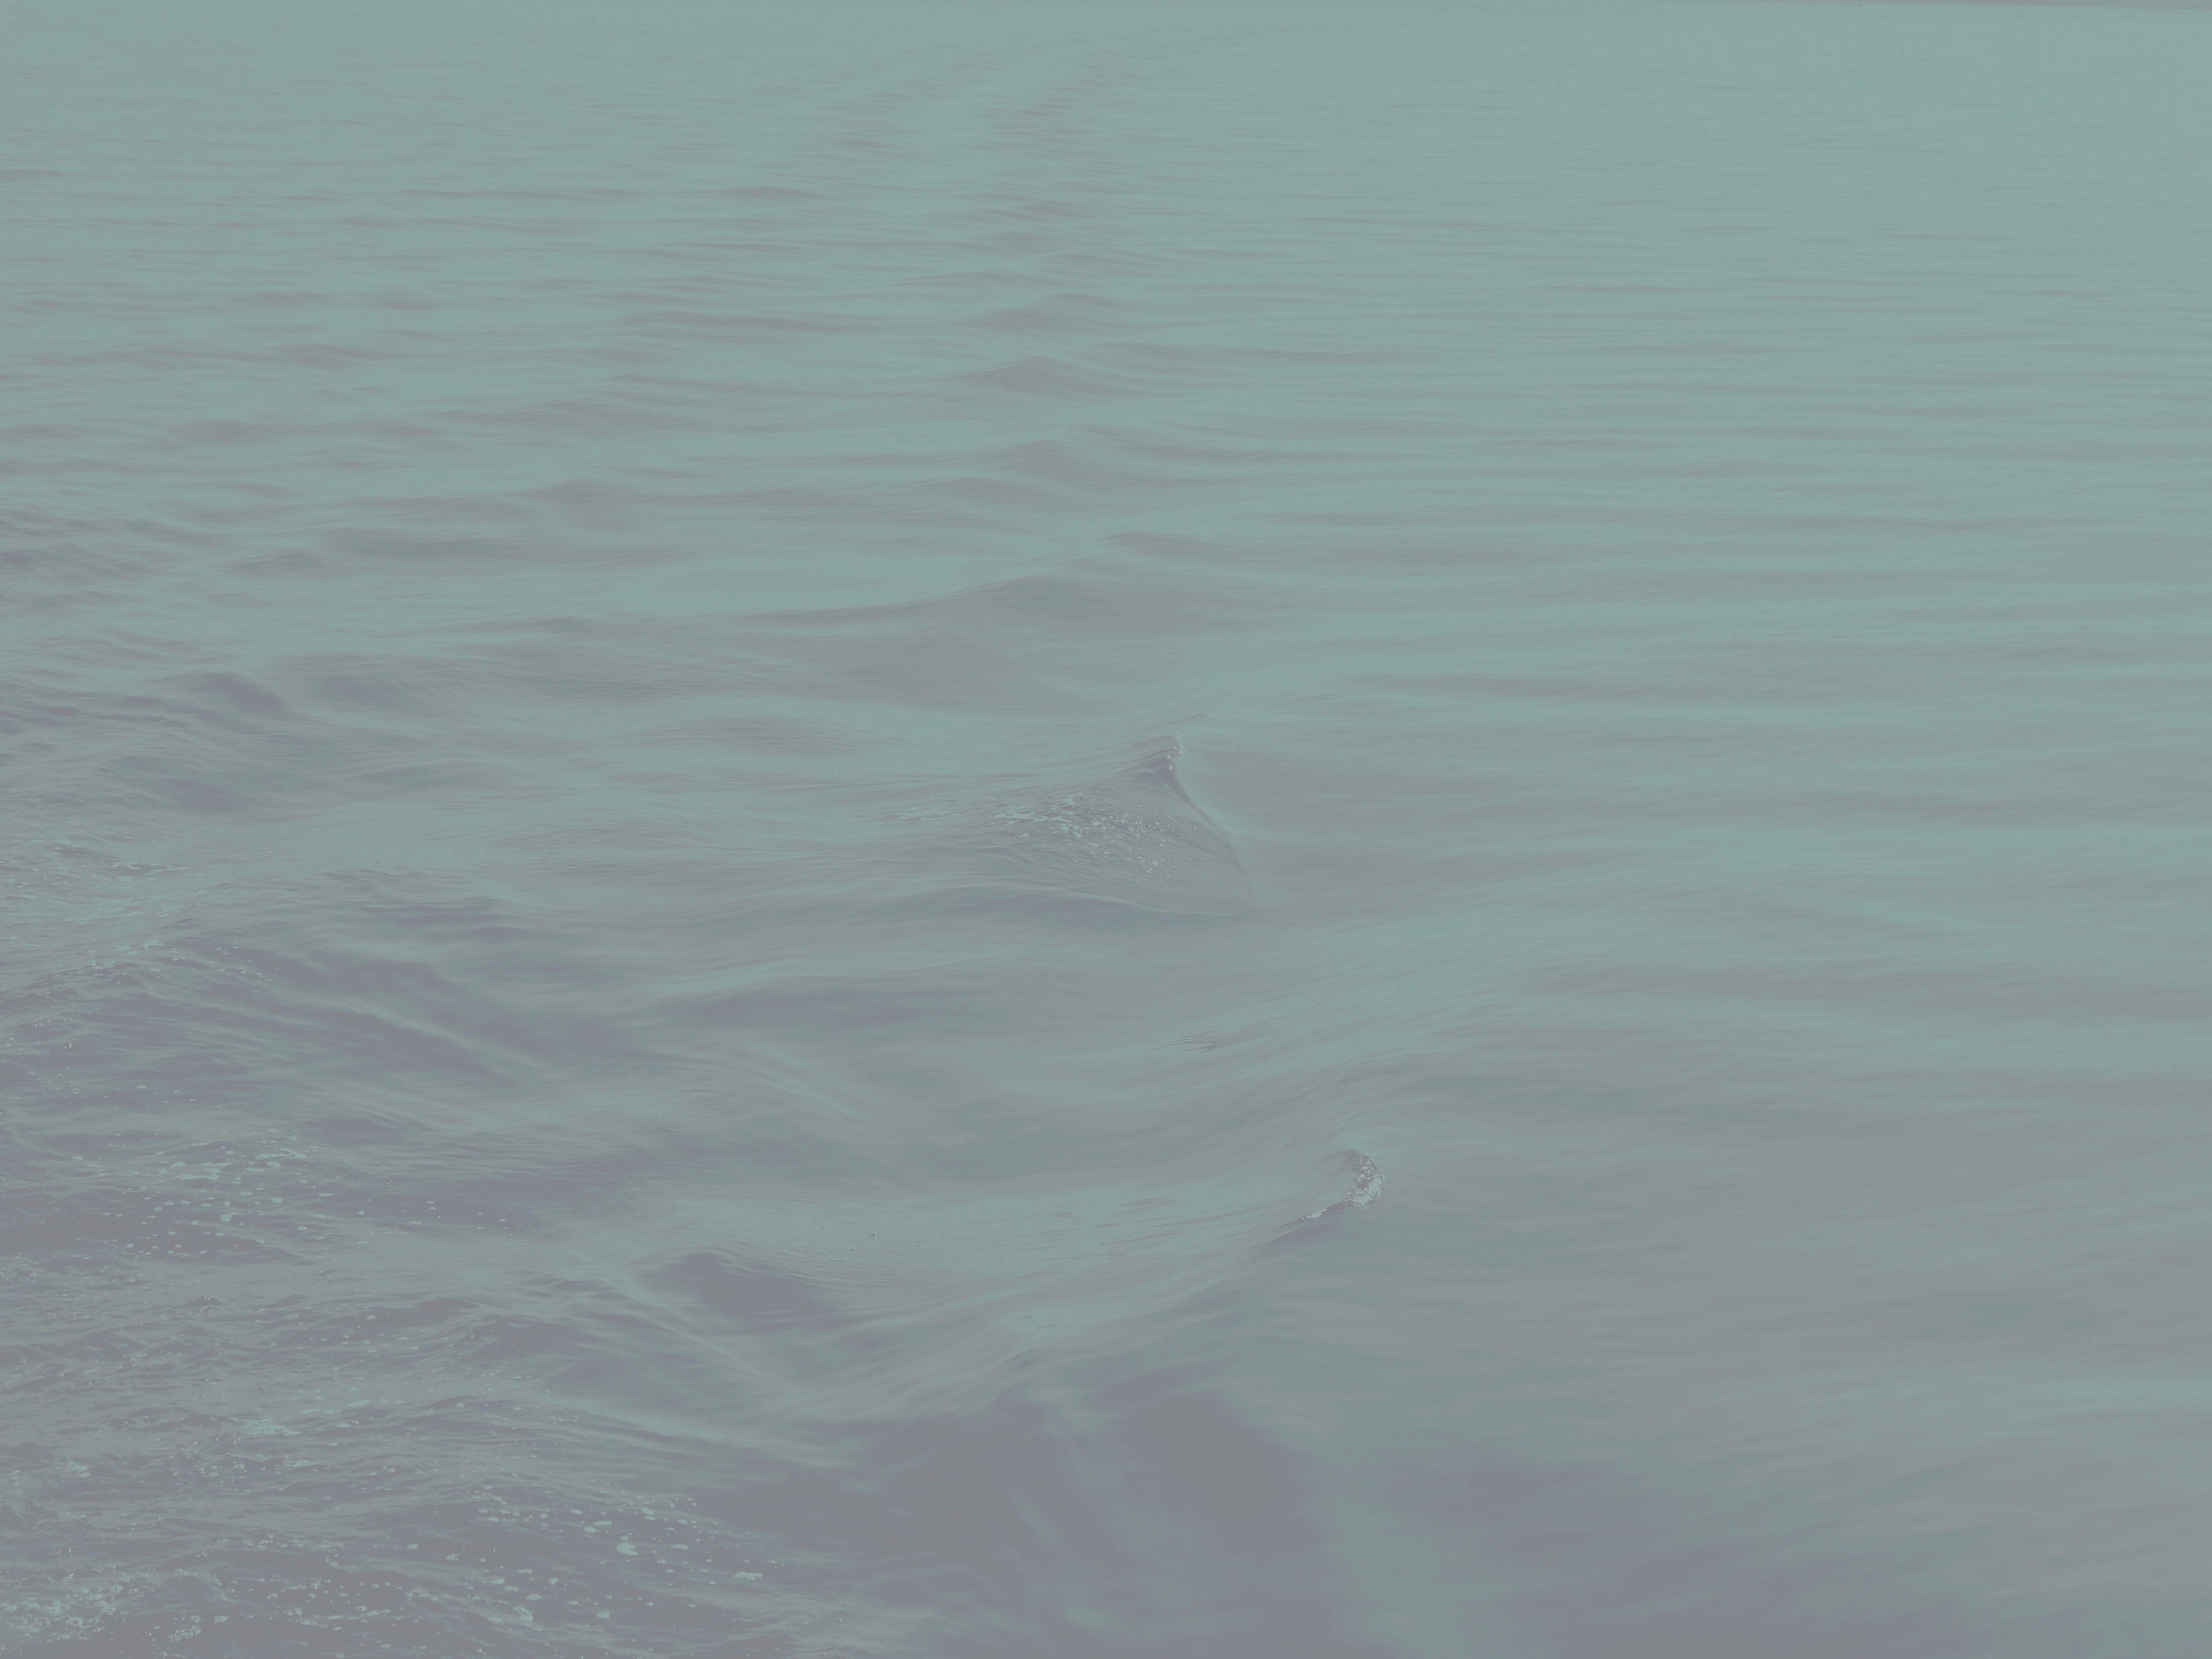
\includegraphics[width=\paperwidth,height=\paperheight]{bklight.jpg}%
}
\setbeamercolor{footline}{fg=textcoldark, bg=imperialblue}
\begin{frame}
\frametitle{\textcolor{textcoldark}{TEST A. Simulate data for LH-LL-V}}
\centering
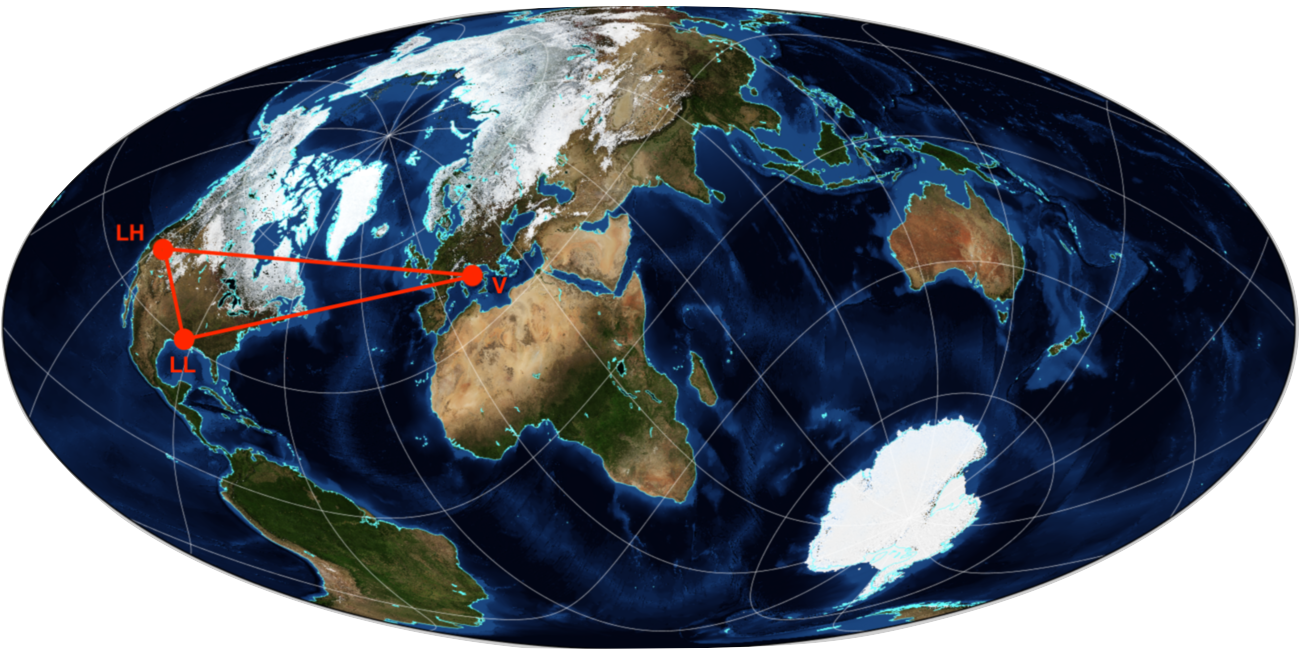
\includegraphics[width=0.95\textwidth]{3b}


\end{frame}

\begin{frame}[plain]
  \vskip 0.7cm
\begin{minipage}{0.061\textwidth}

\vskip -3cm
\textcolor{black}{\Large \bf SNR}
\vskip 1.cm
\centering
\large \textcolor{black}{\centering \bf  0.9
\vskip 2.7cm
\large \bf  0.2}\\
\vskip 2.5cm
\end{minipage}\qquad
\begin{minipage}{0.79\textwidth}
  \Large\qquad \,\,\,\quad\textcolor{black}{ \bf IN}\,\,\,\quad\qquad\qquad\qquad \textcolor{black}{ \bf OUT}
\medskip
 % \vskip -0.7cm
 %\frametitle{Testing the mapper}

 	% \Large \textcolor{black}{ \bfIN}\qquad\qquad\qquad\qquad \textcolor{black}{ \bfOUT}
\centering
 	  \animategraphics[controls,width=\linewidth]{2}{map/maps}{1}{23} %26
 		% remove the 'draft' keyword, when replacing with final figure!
 		\vskip 0.2 cm
 		\footnotesize
 	\textcolor{black}{Strain Intensity [x$10^{{-{43}}}$]}
 	%{Result with 4 dect.s for 15h. Note: the noise in the image is just numerical noise from the inversion. They symmetry of the $\gamma$ makes this reconstruction easy...}

\end{minipage}

%\footnotesize
%Strain Intensity [x$10^{{-{43}}}$]
 \end{frame}

\begin{frame}[plain]
  \vskip 0.7cm
\begin{minipage}{0.061\textwidth}

\vskip -2.3cm
\textcolor{black}{\Large \bf SNR}
\vskip 1.cm
\centering
\large \textcolor{black}{\centering \bf  0.9
\vskip 2.7cm
\large \bf  0.2}\\
\vskip 2.5cm
\end{minipage}\qquad
\begin{minipage}{0.79\textwidth}
  \Large\qquad \,\,\,\quad\textcolor{black}{ \bf IN}\,\,\,\quad\qquad\qquad\qquad \textcolor{black}{ \bf OUT}
\medskip
 % \vskip -0.7cm
 %\frametitle{Testing the mapper}

 	% \Large \textcolor{black}{ \bfIN}\qquad\qquad\qquad\qquad \textcolor{black}{ \bfOUT}
\centering
 	  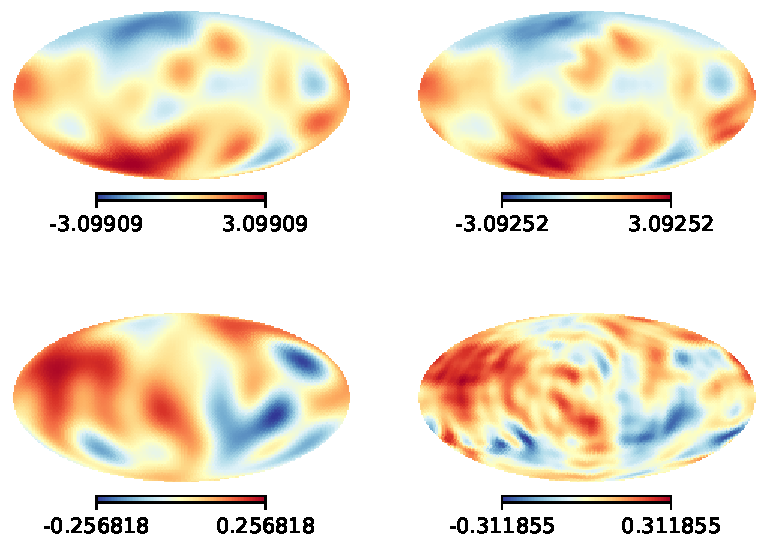
\includegraphics[width=\textwidth]{map/maps23.pdf} %26
 		% remove the 'draft' keyword, when replacing with final figure!
 		\vskip 0.2 cm
 		\footnotesize
 	\textcolor{black}{Strain Intensity [x$10^{{-{43}}}$]}
 	%{Result with 4 dect.s for 15h. Note: the noise in the image is just numerical noise from the inversion. They symmetry of the $\gamma$ makes this reconstruction easy...}

\end{minipage}

%\footnotesize
%Strain Intensity [x$10^{{-{43}}}$]
 \end{frame}

 \begin{frame}
% \vskip -0.2cm
 %\frametitle{Testing the mapper}
\frametitle{\textcolor{textcoldark}{TEST A. Results}}
\Wider{
\centering
\begin{minipage}{0.491\linewidth}
%\centering

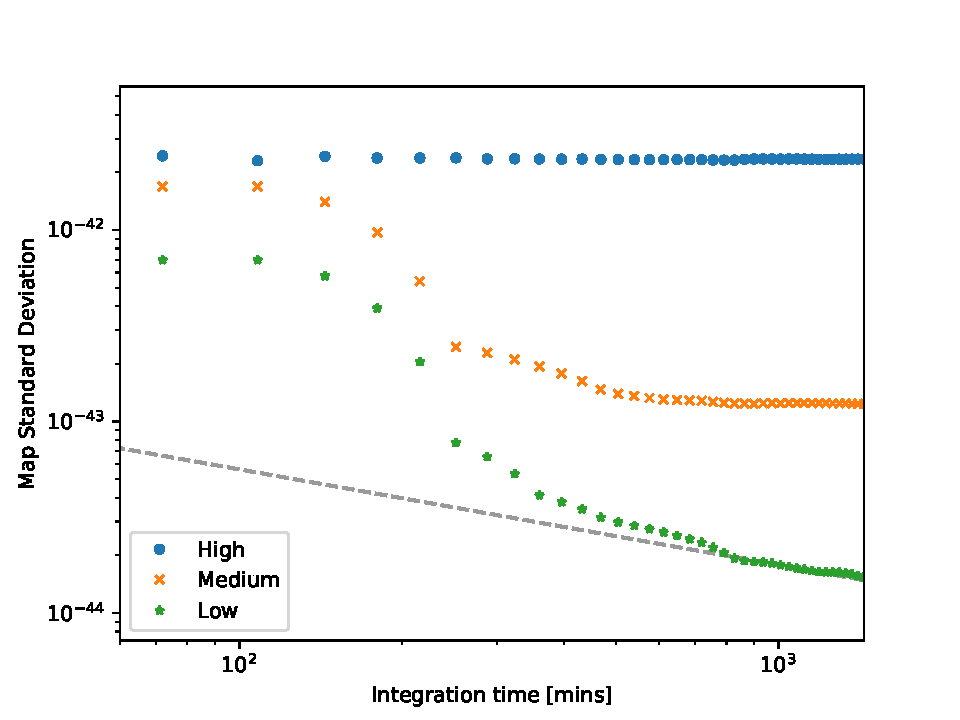
\includegraphics[width=\textwidth]{stds_compare}

\end{minipage}
%\hfill
\begin{minipage}{0.491\linewidth}
%\centering
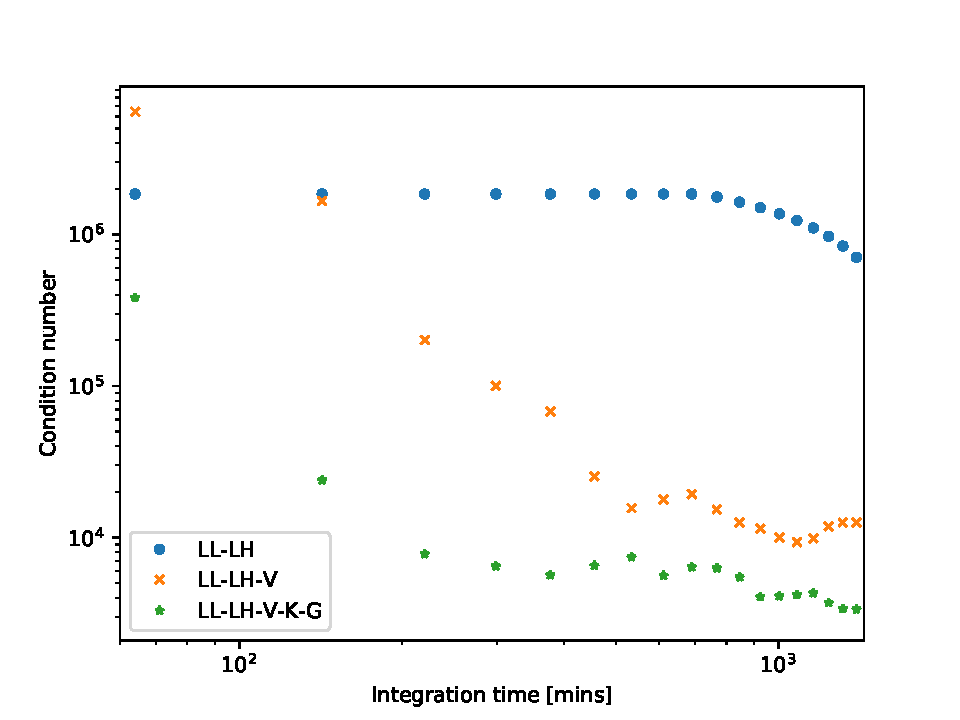
\includegraphics[width=\textwidth]{conds_compare}

\end{minipage}
\small
\flushleft
\textcolor{textcoldark}{
L: Map standard deviation in the LL-LH-V setup for different SNR inputs.\\
\vskip 0.25cm
R: Evolution of condition number of  $\bm A_{mn}$ for different baseline combinations
}
}

 \end{frame}

 \begin{frame}
% \vskip -0.2cm
 %\frametitle{Testing the mapper}
\frametitle{\textcolor{textcoldark}{TEST A. Results}}

\begin{figure}
\centering
\begin{minipage}{0.49\textwidth}
\centering
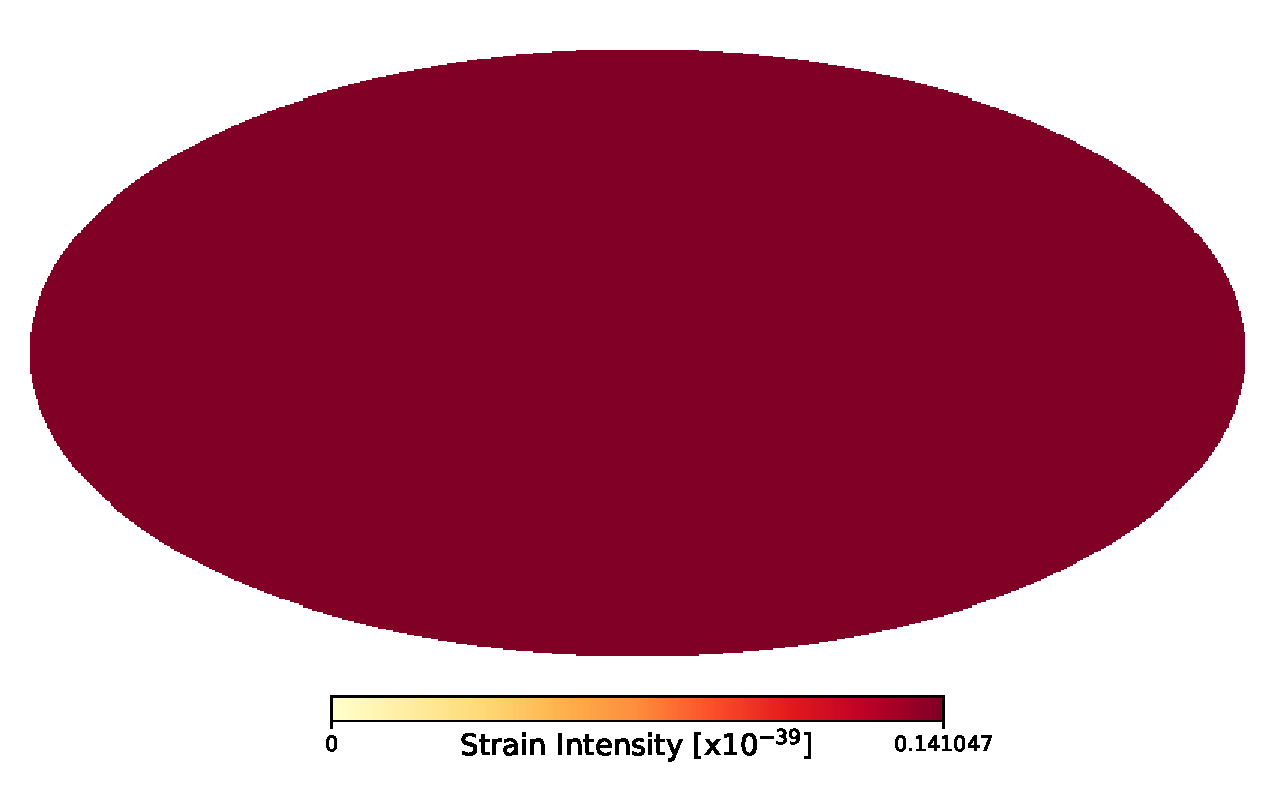
\includegraphics[width=0.9\columnwidth]{1pole1_low}
\end{minipage}\hfill
\begin{minipage}{0.49\textwidth}
\centering
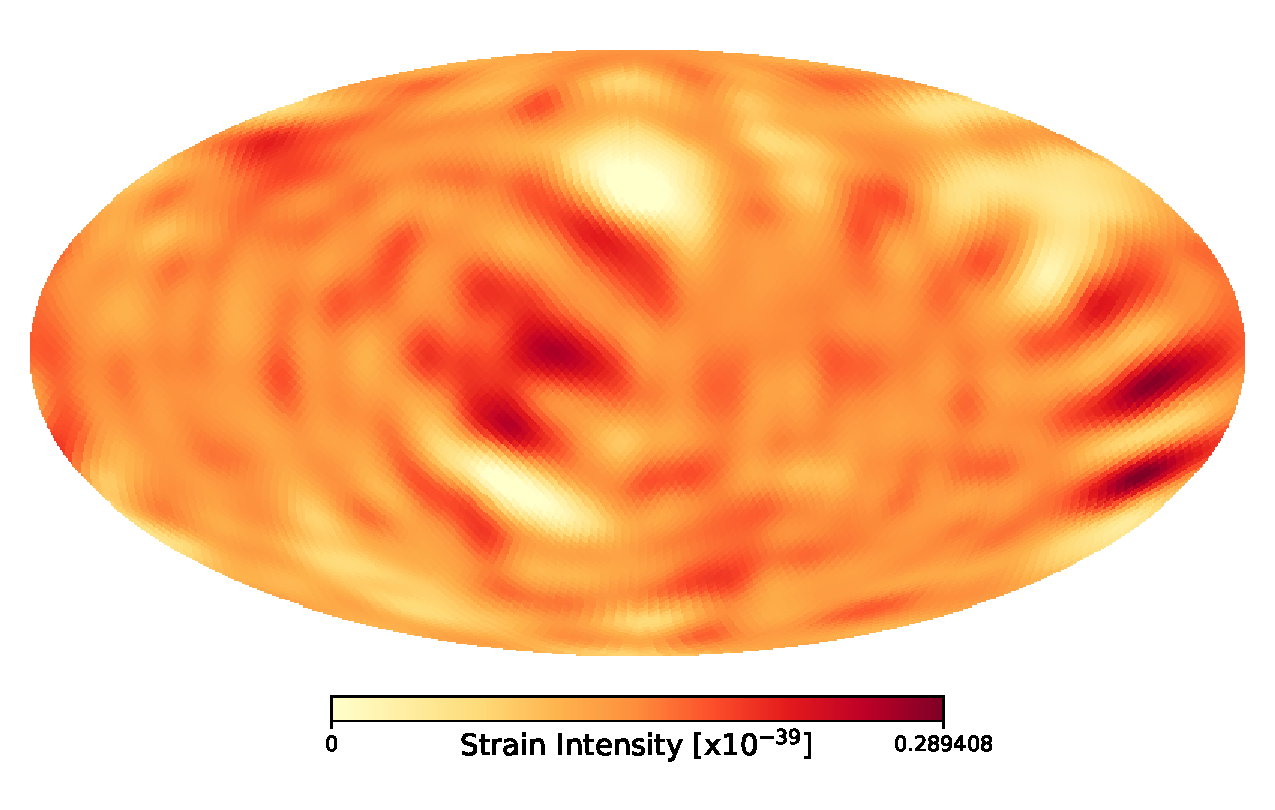
\includegraphics[width=0.9\columnwidth]{1pole2_low}
\end{minipage}\\
\vskip 0.5 cm
\begin{minipage}{0.49\textwidth}
\centering
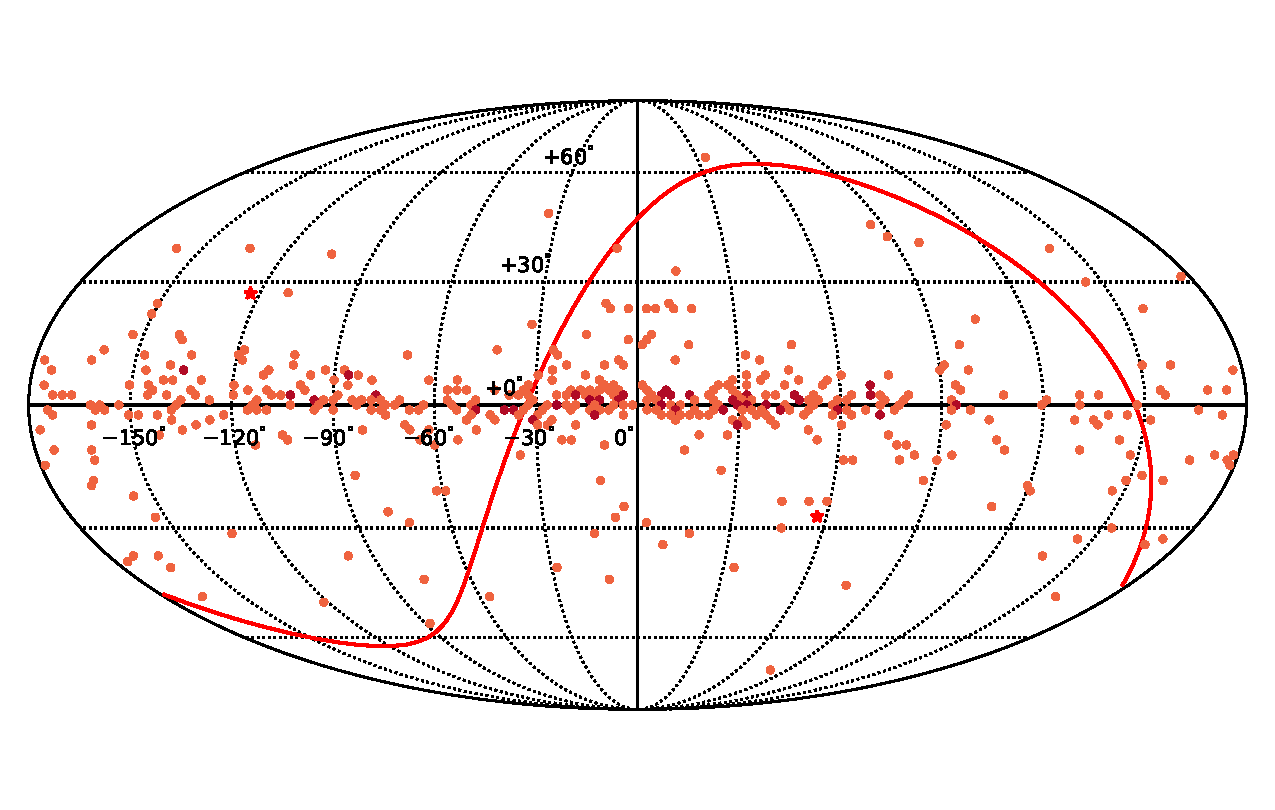
\includegraphics[width=0.9\columnwidth]{map_poi}
\end{minipage}\hfill
\begin{minipage}{0.49\textwidth}
\centering
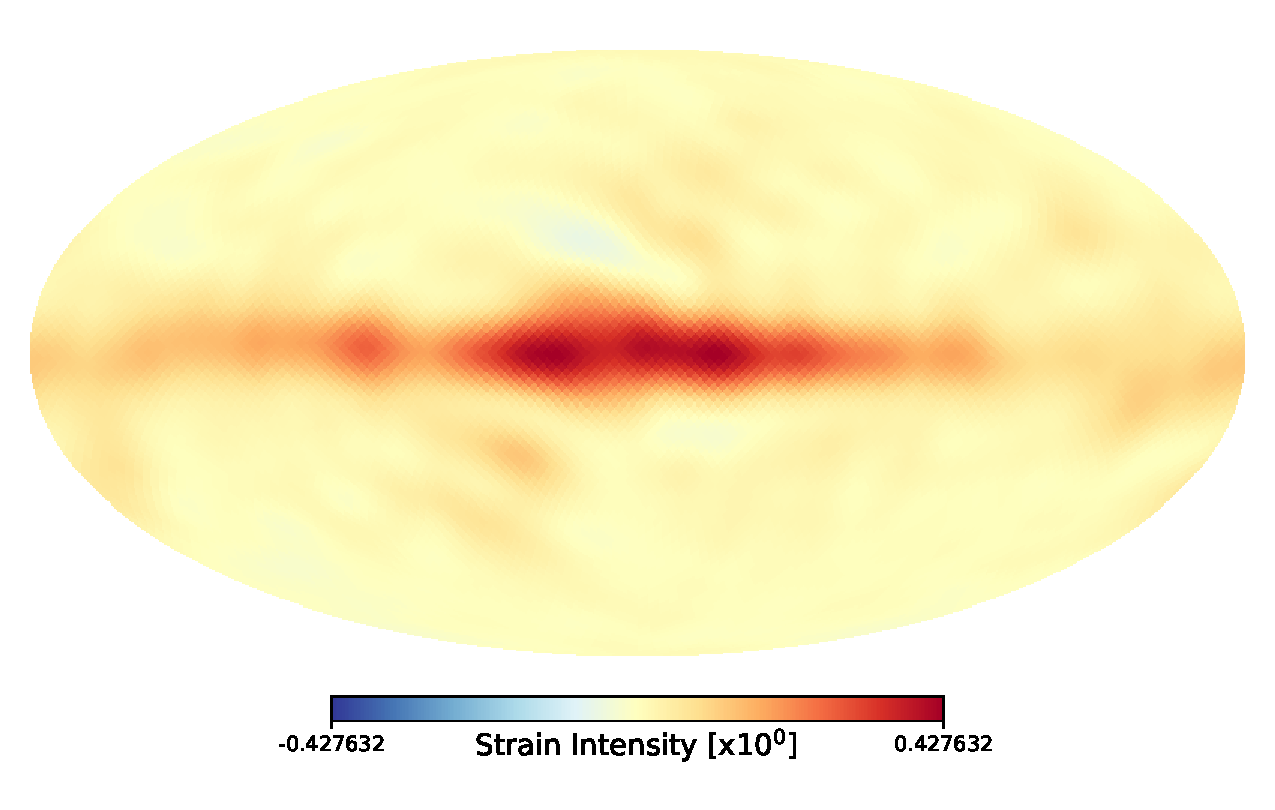
\includegraphics[width=0.9\columnwidth]{planck_poi_high}
\end{minipage}
\caption*{\textcolor{black}{Simulations in different SNR regimes and for different input maps.}}
\label{fig:stdev_sim}
\end{figure}

 \end{frame}


 \begin{frame}

 \frametitle{\textcolor{textcoldark}{TEST B. Analyse LIGO O1 run}}
 %\vskip -0.2cm
 %\frametitle{Testing the mapper}
 	\begin{figure}
 	   \animategraphics[controls,width=0.9\linewidth]{2}{LIGO/LIGOmap}{0}{29} %26
 		% remove the 'draft' keyword, when replacing with final figure!
 		\medskip\\
 	%\caption*{\Large LIGO O1 data, ~1 week \normalsize \textcolor{red}{\bf -- full run soon}}
 	%{Result with 4 dect.s for 15h. Note: the noise in the image is just numerical noise from the inversion. They symmetry of the $\gamma$ makes this reconstruction easy...}
 	\scriptsize
 	\textcolor{black}{framerate $\sim$ 1.5 days/frame}
 	\end{figure}

 \end{frame}
  \begin{frame}

 \frametitle{\textcolor{textcoldark}{TEST B. Analyse LIGO O1 run}}
 %\vskip -0.2cm
 %\frametitle{Testing the mapper}
 	\begin{figure}
 	   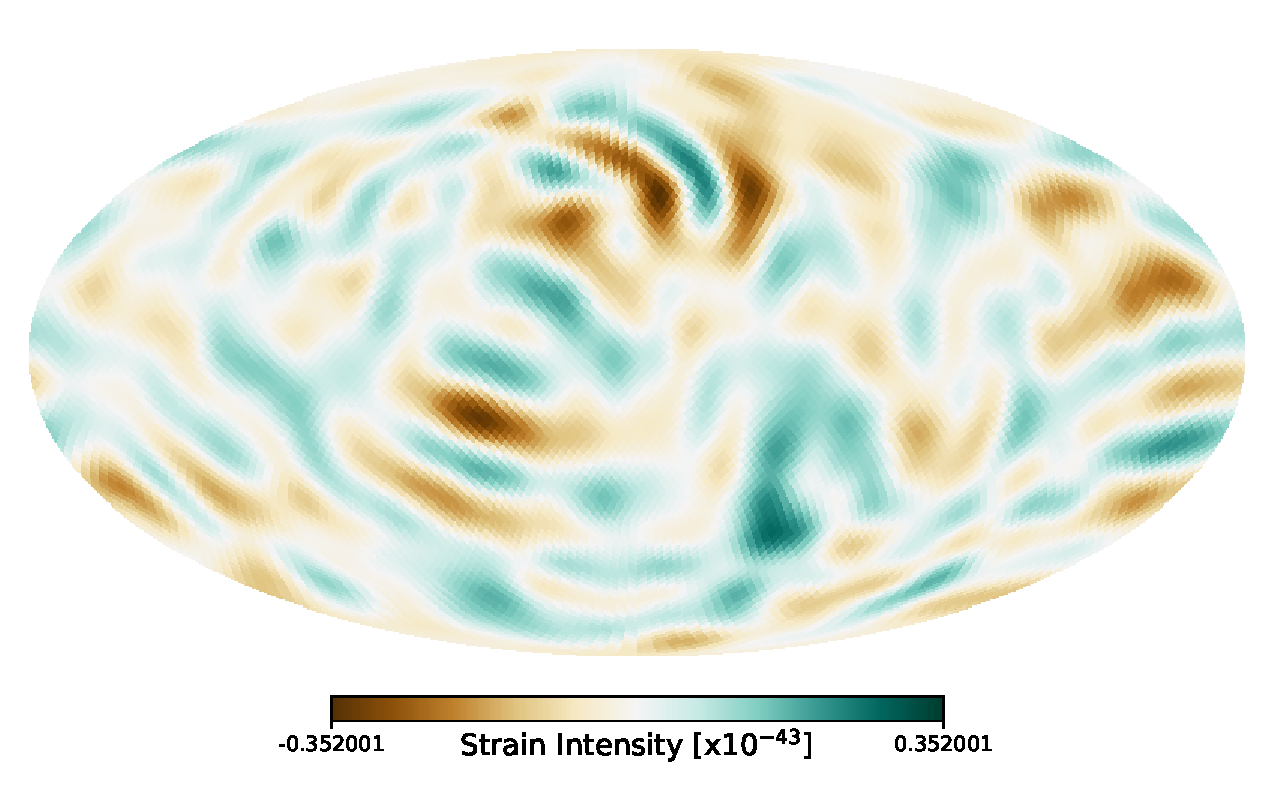
\includegraphics[width=0.9\textwidth]{LIGO/LIGOmap29.pdf} %26
 		% remove the 'draft' keyword, when replacing with final figure!
 		\smallskip
 	%\caption*{\Large LIGO O1 data, ~1 week \normalsize \textcolor{red}{\bf -- full run soon}}
 	%{Result with 4 dect.s for 15h. Note: the noise in the image is just numerical noise from the inversion. They symmetry of the $\gamma$ makes this reconstruction easy...}
 	\end{figure}

 \end{frame}
 
 \begin{frame}
\frametitle{\textcolor{textcoldark}{TEST B. Results}}
\vskip 0.35 cm
\centering
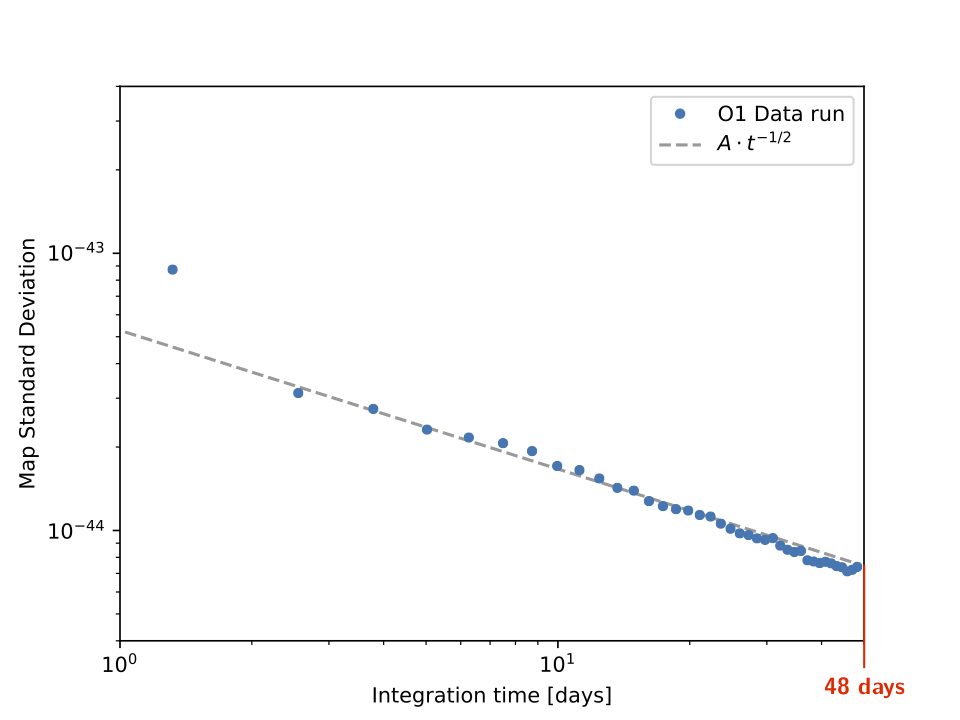
\includegraphics[width=0.9\textwidth]{fits_stds_zoom.jpg}


\end{frame}

 \begin{frame}
\frametitle{\textcolor{textcoldark}{TEST B. Results}}
\vskip 0.35 cm
\normalsize
\textcolor{black}{We found that the standard deviation of the recovered maps of the GWB is steadily decreasing $\sim t^{-1/2}$ $\Rightarrow$ {\bf consistent with noise}.\\
\smallskip
The assumed spectral dependence is 
$$
I_{GW} \propto f^0 \qquad \Rightarrow \qquad \Omega_{GW} \propto f^{3}
$$
consistent with an astrophysical background.\\
\medskip
Our estimate at 95\% CL on the AGWB is }
\begin{block}{}
\centering
\textcolor{textcol}{$\bm{\Omega_{\bm GW} < \bm 3.8 \times 10^{-8}}$}
\end{block}
\textcolor{black}{
this is a rough estimate as it is not weighted by the noise covariance of the map, but it is a good reality check.
}

\end{frame}

}

\begin{frame}[plain]
\LARGE
\textcolor{textcol}{\bf Next steps:}\\
\large
\bigskip
\bigskip
\begin{itemize}
    \item[$\bigstar$] \textcolor{white}{Analyse O1 data with different spectral laws (eg. for CGWB)}\hfill
    \item[$\bigstar$] \textcolor{white}{ Include polarisation reconstruction (Q, U, V)}
    \item[$\bigstar$] \textcolor{white}{ Generalize to other detector types: LISA, PTAs}
    \item[$\bigstar$] \textcolor{white}{ Produce model-based input maps and test reconstruction}
\end{itemize}
%LISA is expected to probe extensively the frequency range for the AGWB... good news!
\medskip
\Large

\begin{center}
\textbf{\textcolor{textcol}{Thank you for listening!}}
\end{center}
\end{frame}


\end{document}

